\documentclass[12pt]{article}

% This is the preamble, load any packages you're going to use here
\usepackage{physics} % provides lots of nice features and commands often used in physics, it also loads some other packages (like AMSmath)
\usepackage{siunitx} % typesets numbers with units very nicely
\usepackage{enumerate} % allows us to customize our lists
\usepackage{titlesec}
\usepackage{amsmath}
\usepackage{geometry}
\usepackage{listings}
\usepackage{xcolor} % for setting colors
\usepackage{graphicx}
\usepackage{subcaption}
\usepackage{hyperref}

\lstset{
  language=Matlab,
  basicstyle=\ttfamily\scriptsize, % smaller font size
  keywordstyle=\color{blue},
  stringstyle=\color{red},
  commentstyle=\color{gray}, % grey color for comments
  morecomment=[l][\color{magenta}]{\#},
  frame=single,
  breaklines=true,
  numbers=left,
  numberstyle=\tiny\color{gray},
  stepnumber=1,
  numbersep=10pt,
  backgroundcolor=\color{white},
  tabsize=4,
  showspaces=false,
  showstringspaces=false
}



\titleformat*{\section}{\large\bfseries}
\titleformat*{\subsection}{\small\bfseries}



\begin{document}

\title{Optical Wireless Communication System \\ \large{Final Assignment - NTUST Short Course}}
\author{Martin Clinton Manullang (D10902809)}
\date{\today}
\maketitle

This \LaTeX\  document, including all graphics, code and content can be accessed from \href{https://github.com/mctosima/OWC-NottinghamNTUST-FinalAssignment/tree/main}{this repository}.

\section{Visible Light Communication}
	In this problem, we want to simulate the 3D receieved power based on the given condition below (The variable in the MATLAB script denoted in the bracket):
    \begin{itemize}
        \item LED Power (\texttt{P\_LED}) = $2 \text{W}$
        \item LED Beam Profile (\texttt{ml}) = 1 to 20 (This is looped from 1 to 20)
        \item Receiver Photodetector Size (\texttt{Adet}) = $1 * 10^-{4}$
        \item Field of View of the Receiver (\texttt{FOV}) = $140^\circ$
        \item Room Size / Space Size: width * length * height (\texttt{lx, ly, h}) = $2 \text{m} * 2 \text{m} * 3 \text{m}$
        \item Position of LED at center of room (\texttt{XT, YT}) = $0 \text{m} , 0 \text{m}$
    \end{itemize}

    The above parameters is written down in the MATLAB script as below:

    \begin{lstlisting}
    P_LED = 2; % transmitted optical power by individual LED
    Adet = 1 * 10 ^ -4; % detector physical area of a PD
    Ts = 1; % gain of an optical filter
    index = 1.5; % refractive index of a lens at a PD
    FOV = 140; % FOV of a receiver
    G_Con = (index ^ 2) / (sind(FOV) .^ 2); % gain of an optical concentrator
    lx = 2; ly = 2; h = 3; % room dimensions in meters
    XT = 0; YT = 0; % Position of the single LED
    resolution = 20;
    Nx = lx * resolution; Ny = ly * resolution;
    x = linspace(-lx / 2, lx / 2, Nx);
    y = linspace(-ly / 2, ly / 2, Ny);
    [XR, YR] = meshgrid(x, y);
    \end{lstlisting}

    \subsection{Plot of 3D receieved power}
    Instead of plotting for \texttt{ml = 1} and \texttt{ml = 20}, I iterate the loop from \texttt{ml = 1} to \texttt{ml = 20} to make it easier to answer the next question.

    Here's the plot results of \texttt{ml = 1} and \texttt{ml = 20} in Watt and dBm:

    \begin{figure}[htbp]
        \centering
        \begin{subfigure}[b]{0.45\textwidth}
            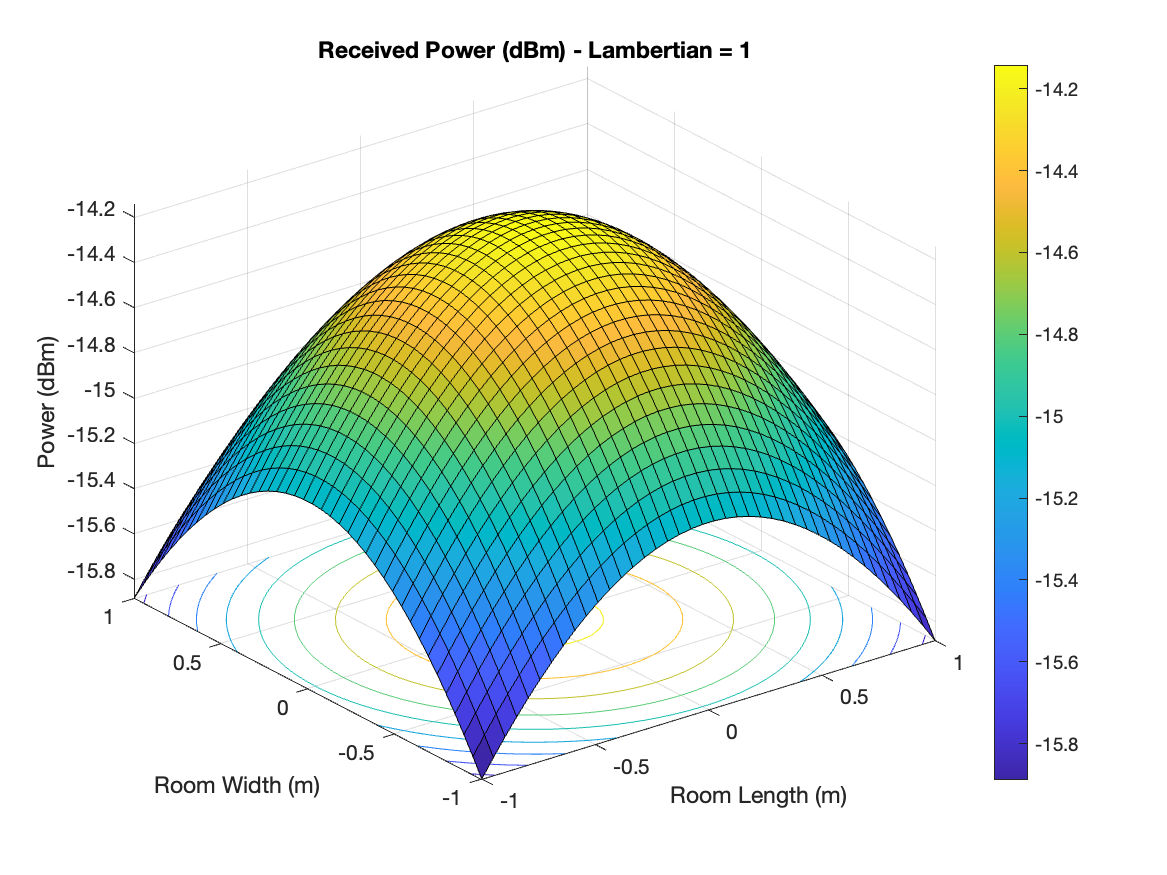
\includegraphics[width=\textwidth]{images/3D_power_curve_dBm_1.png}
            \caption{Power Curve (dBm)}
            \label{fig:power_curve_dBm}
        \end{subfigure}
        \hfill
        \begin{subfigure}[b]{0.45\textwidth}
            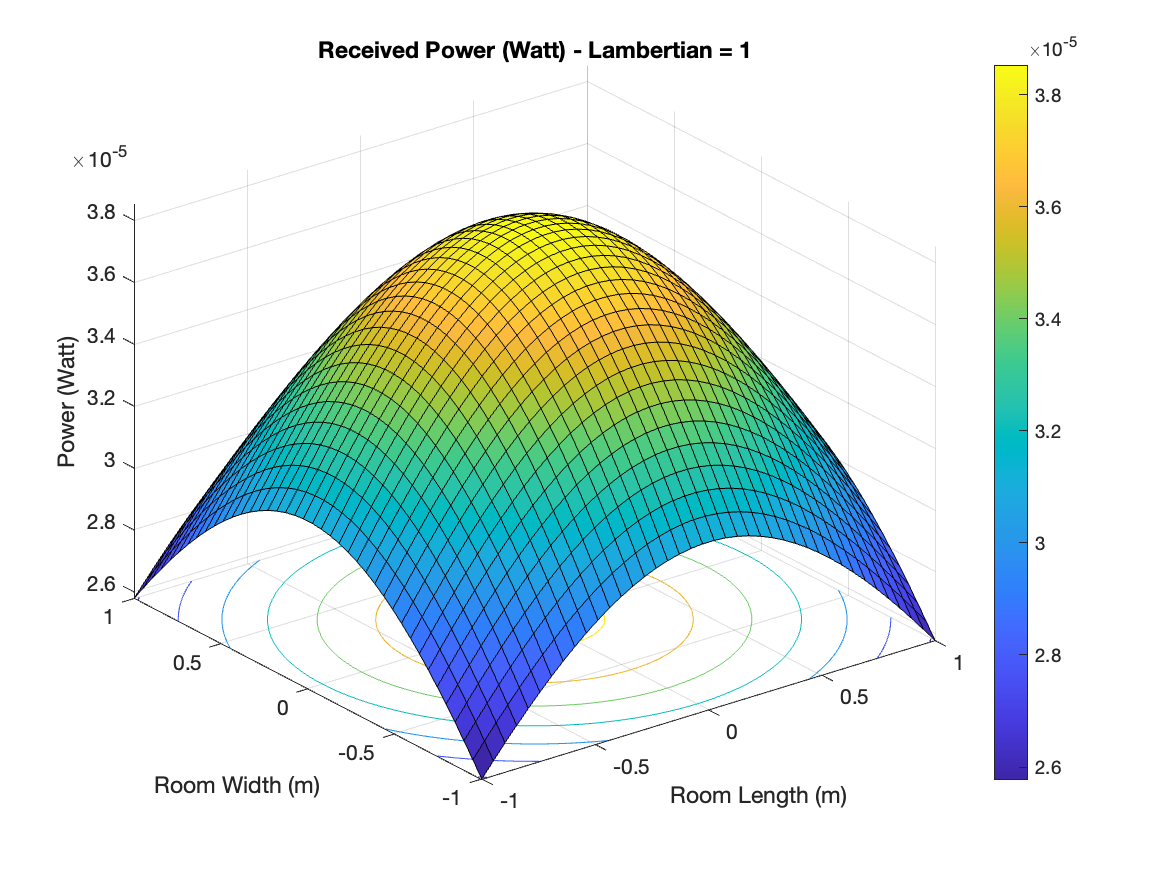
\includegraphics[width=\textwidth]{images/3D_power_curve_Watt_1.png}
            \caption{Power Curve (Watt)}
            \label{fig:power_curve_Watt}
        \end{subfigure}
        \caption{Side-by-side plot of power curves with \texttt{ml = 1}}
        \label{fig:power_curves}
    \end{figure}

    \begin{figure}[htbp]
        \centering
        \begin{subfigure}[b]{0.45\textwidth}
            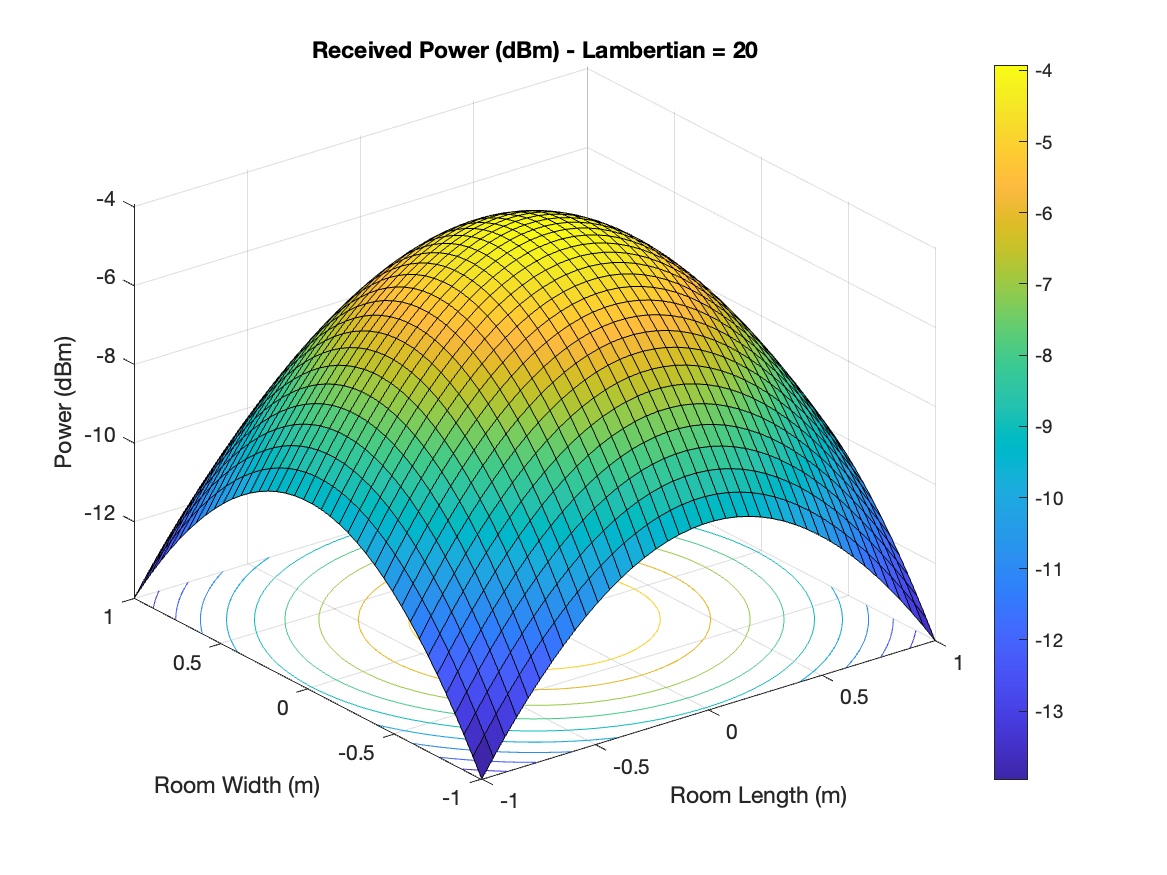
\includegraphics[width=\textwidth]{images/3D_power_curve_dBm_20.png}
            \caption{Power Curve (dBm)}
            \label{fig:power_curve_dBm}
        \end{subfigure}
        \hfill
        \begin{subfigure}[b]{0.45\textwidth}
            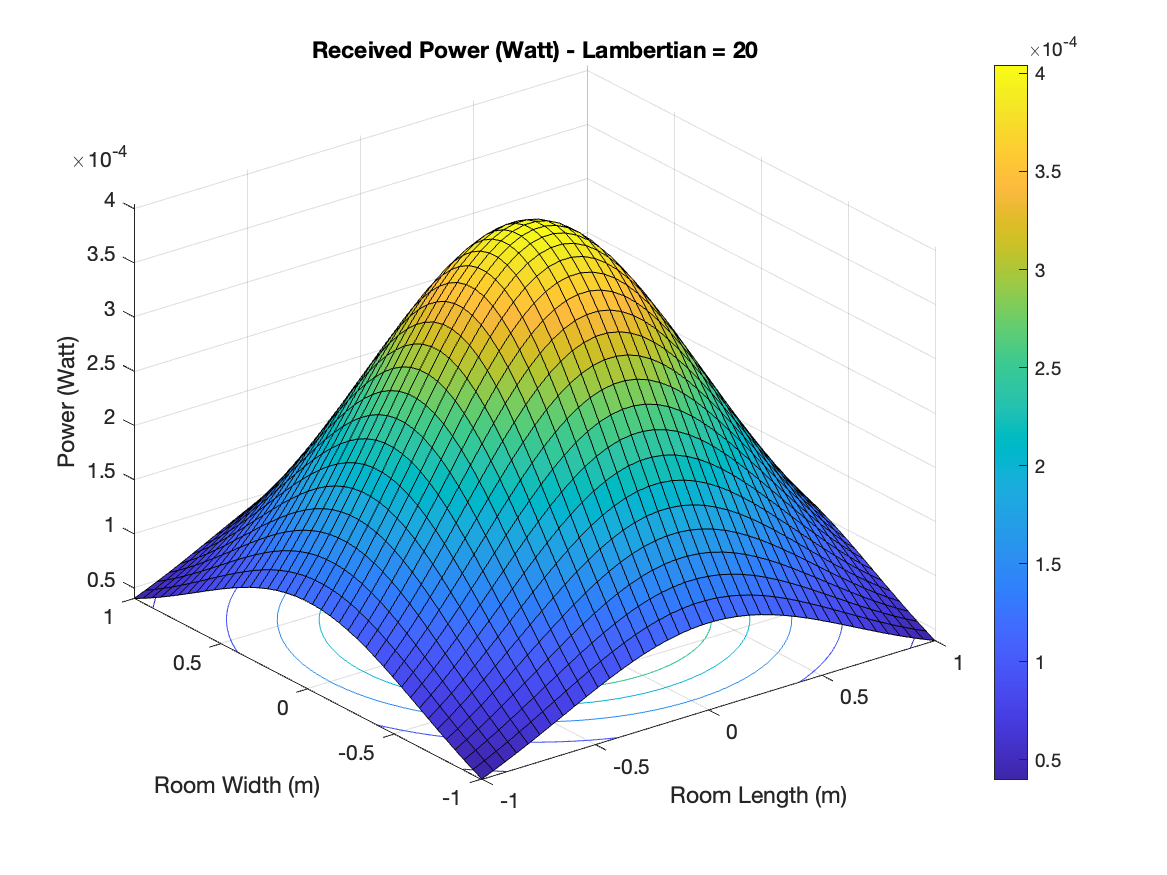
\includegraphics[width=\textwidth]{images/3D_power_curve_Watt_20.png}
            \caption{Power Curve (Watt)}
            \label{fig:power_curve_Watt}
        \end{subfigure}
        \caption{Side-by-side plot of power curves with \texttt{ml = 20}}
        \label{fig:power_curves}
    \end{figure}

    \subsection{Optimum Lambertian Order}

    To answer this question, we modify our script to store the power at the center and corner for every \texttt{ml} from 1 to 20 as follows:

    \begin{lstlisting}
    for ml = 1:20 % Lambertian order range

        D = sqrt((XR - XT) .^ 2 + (YR - YT) .^ 2 + h ^ 2); % Distance vector
        cosphi = h ./ D; % Angle vector
        receiver_angle = acosd(cosphi);
        H = (ml + 1) * Adet .* cosphi .^ (ml + 1) ./ (2 * pi .* D .^ 2); % Channel DC gain
        P_rec = P_LED .* H .* Ts .* G_Con; % Received power
        P_rec(abs(receiver_angle) > FOV) = 0;
        P_rec_dBm = 10 * log10(P_rec * 1000);
    
        % Find the received power at the center and one of the corners
        P_center = P_rec(Ny/2, Nx/2); % Center of the room
        P_corner = P_rec(1, 1); % Top-left corner of the room
    
        % Convert powers to dBm for comparison
        P_center_dBm = 10 * log10(P_center * 1000);
        P_corner_dBm = 10 * log10(P_corner * 1000);
    
        % Store the powers for each Lambertian order
        power_at_center = [power_at_center P_center_dBm];
        power_at_corner = [power_at_corner P_corner_dBm];
    
        % Plot in Watt
        figure(1)
        surfc(x, y, P_rec);
        xlabel('Room Length (m)');
        ylabel('Room Width (m)');
        zlabel('Power (Watt)');
        title(['Received Power (Watt) - Lambertian = ', num2str(ml)]);
        colorbar
        drawnow
        % Save as PNG and SVG
        saveas(gcf, ['3D_power_curve_Watt_', num2str(ml), '.png']);
        saveas(gcf, ['3D_power_curve_Watt_', num2str(ml), '.svg']);
        % Append to GIF
        frame = getframe(gcf);
        im = frame2im(frame);
        [imind, cm] = rgb2ind(im, 256);
        if ml == 1
            imwrite(imind, cm, filenameWatt, 'gif', 'Loopcount', inf, 'DelayTime', 0.5);
        else
            imwrite(imind, cm, filenameWatt, 'gif', 'WriteMode', 'append', 'DelayTime', 0.5);
        end
    
        % Plot in dBm
        figure(2)
        surfc(x, y, P_rec_dBm);
        xlabel('Room Length (m)');
        ylabel('Room Width (m)');
        zlabel('Power (dBm)');
        title(['Received Power (dBm) - Lambertian = ', num2str(ml)]);
        colorbar
        drawnow
        % Save as PNG and SVG
        saveas(gcf, ['3D_power_curve_dBm_', num2str(ml), '.png']);
        saveas(gcf, ['3D_power_curve_dBm_', num2str(ml), '.svg']);
        % Append to GIF
        frame = getframe(gcf);
        im = frame2im(frame);
        [imind, cm] = rgb2ind(im, 256);
        if ml == 1
            imwrite(imind, cm, filenameDBm, 'gif', 'Loopcount', inf, 'DelayTime', 0.5);
        else
            imwrite(imind, cm, filenameDBm, 'gif', 'WriteMode', 'append', 'DelayTime', 0.5);
        end
    end
    
    % Find the difference that close to 6 dB between the center and the corner
    power_difference = power_at_center - power_at_corner;
    % Find the Lambertian order that gives the closest to 6 dB difference
    [~, index] = min(abs(power_difference - 6));
    
    fprintf('The Lambertian order that gives the closest to 6 dB difference is %d\n', index);
    fprintf('The received power at the center is %f dBm\n', power_at_center(index));
    fprintf('The received power at the corner is %f dBm\n', power_at_corner(index));
    fprintf('The difference between the center and the corner is %f dB\n', power_difference(index));
    \end{lstlisting}

    At the end of the code, we obtained the result as below:

    \begin{itemize}
        \item The Lambertian order that gives the closest to 6 dB difference is 11
        \item The received power when \texttt{ml = 11} at the center is -6.366077 dBm
        \item The received power when \texttt{ml = 11} at the corner is -12.462148 dBm
        \item The difference when \texttt{ml = 11} between the center and the corner is 6.096071 dB
    \end{itemize}

    I also tried to animate the changes and save it as .gif files that can be seen on this link below:
    \begin{itemize}
        \item \href{https://raw.githubusercontent.com/mctosima/OWC-NottinghamNTUST-FinalAssignment/main/3D_power_curve_Watt.gif}{Watt}
        \item \href{https://raw.githubusercontent.com/mctosima/OWC-NottinghamNTUST-FinalAssignment/main/3D_power_curve_dBm.gif}{dBm}
    \end{itemize}
    
    
\section{Free Space Optical Wireless Communications}
\subsection{The link budget in clear weather condition}
		From the question, we obtain some value such below:
\begin{itemize}
    \item $\textit{L} = 1.2\, \text{km} = 1200\, \text{m}$
    \item $\gamma_{t}(\lambda) = 0.4\, \text{km}^{-1}$
    \item $\alpha = 0.2\,^\circ = 0.0035\, \text{rad}$
    \item $P_{t} = 40\, \text{mW} = 16.0206\, \text{dBm}$
    \item $\textit{r} = 30\, \text{cm} = 0.3\, \text{m}$
    \item $\textit{rec}_{sens} = -30\, \text{dBm}$
\end{itemize}

First, we calculate the atmospheric Loss as below:

    \begin{equation}
    \text{atm\_loss} = \exp(-0.4\, \text{km}^{-1} \times 1.2\, \text{km}) = 0.6188\, \text{mW} = -2.0846\, \text{dB}
    \end{equation}

Next, we calculate the geometry loss. Before that, we need to get the coverage area and the collection area.

    \begin{equation}
    \text{coverage\_area} = \pi \times (1200 \times \tan(\frac{0.0035}{2})^2) \\
    = 13.7806
    \end{equation}

    \begin{equation}
    \text{collection\_area} = \pi \times (0.3)^2 = 0.2827
    \end{equation}

Then, we can calculate the geometry loss as below:

    \begin{equation}
    \text{geometry\_loss} = \frac{\text{collection\_area}}{\text{coverage\_area}} = 0.0205\, \text{mW} = -16.8788 \text{dB}
    \end{equation}

Finally, we have all of the value to calculate the link budget. Which are:
    \begin{itemize}
        \item $P_{t} = 40\, \text{mW} = 16.0206\, \text{dBm}$
        \item $\text{atm\_loss} = 0.6188\, \text{mW} = -2.0846\, \text{dB}$
        \item $\text{geometry\_loss} = 0.0205\, \text{mW} = -16.8788 \text{dB}$
        \item $\textit{rec}_{sens} = -30\, \text{dBm}$
    \end{itemize}

    \begin{equation}
        \begin{split}
            \text{link\_budget} &= P_{t} + \text{atm\_loss} + \text{geometry\_loss} - \textit{rec}_{sens} \\
            &= 16.0206\, \text{dBm} + (-2.0846\, \text{dB}) + (-16.8788 \text{dB}) - (-30\, \text{dBm}) \\
            &= 27.06\, \text{dB}
        \end{split}
    \end{equation}

\subsection{The link budget in foggy weather condition}

Given the Figure 2, we obtained the moderate fog visibility 500m is having $\gamma_{t}(\lambda) = 28.9 \text{db/Km}$. By using that, we can calculate the fog loss as below:

\begin{equation}
    \text{fog\_loss} = 28.9 \times 1.2 = 34.68\, \text{dB}
\end{equation}

Finally, we can calculate the available link power on foggy weather condition as follows:

    \begin{equation}
        \begin{split}
            \text{available\_link\_power} &= \text{link\_budget} - \text{fog\_loss} \\
            &= 27.06\, \text{dB} - 34.68\, \text{dB} \\
            &= -7.62\, \text{dB}
        \end{split}
    \end{equation}

We can conclude that the available link power on foggy weather condition is $-7.62\, \text{dB}$ which is insufficient to support the link.


\newpage
\appendix

\section*{Appendix A - First Matlab Code}
\lstinputlisting{task1.m}

\section*{Appendix B - Second Matlab Code}
\lstinputlisting{task2.m}
        




\end{document}